\documentclass{report}
\usepackage{textcase}
\usepackage{amsmath}
\usepackage{amsfonts}
\usepackage{amssymb}
\usepackage[utf8]{vietnam}
\usepackage{graphicx}
\usepackage{scrextend}
\usepackage[left=3.5cm,right=2cm,top=3.5cm,bottom=3cm]{geometry}
\usepackage{xhfill}
\usepackage{floatrow}
\usepackage{subfigure}
\usepackage{wrapfig}
\usepackage{lipsum}
\usepackage{lettrine}
\usepackage[
    backend=biber,
    style=authoryear,
    natbib=true,
    url=true, 
    doi=true,
    eprint=false
]{biblatex}
\usepackage{hyperref} 
\addbibresource{myref.bib}

\begin{document}
\newcommand{\xfill}[2][1ex]{{%
  \dimen0=#2\advance\dimen0 by #1
  \leaders\hrule height \dimen0 depth -#1\hfill%
}}

%Page 1
\changefontsizes[14pt]{12pt}
\centerline{TỔNG LIÊN ĐOÀN LAO ĐỘNG VIỆT NAM}

\changefontsizes[14pt]{11pt}
\centerline{\textbf{TRƯỜNG ĐẠI HỌC TÔN ĐỨC THẮNG}}
\centerline{\textbf{KHOA CÔNG NGHỆ THÔNG TIN}}

\begin{center}
    \begin{figure}[htp]
    \begin{center}
     
\includegraphics[scale=.2]{logo}
    \end{center}
    \end{figure}
\end{center}

\changefontsizes{16pt}
\centerline{\textbf{ĐỒ ÁN: LẬP TRÌNH WEB VÀ ỨNG DỤNG}}
\vspace{1.5cm}
\changefontsizes{24pt}
\centerline{\textbf{WEBSITE XEM PHIM TRỰC TUYẾN}}

\vspace{4cm}
\begin{flushright}
\renewcommand{\baselinestretch}{0.05}
\changefontsizes{14pt}
\textit{Người hướng dẫn: }\textbf{G.V Đặng Minh Thắng}
\setlength{\parskip}{0.5em}

\textit{Người thực hiện: }\textbf{Trần Quốc Lĩnh - 51703124}
\setlength{\parskip}{0.5em}

Lớp: \textbf{17050301}
\setlength{\parskip}{0.5em}

Khoá: \textbf{21}
\setlength{\parskip}{0.5em}

\end{flushright}

\vspace{1cm}
\changefontsizes{14pt}
\centerline{\textbf{THÀNH PHỐ HỒ CHÍ MINH, NĂM 2019}}


%Page 2
\changefontsizes[14pt]{12pt}
\centerline{TỔNG LIÊN ĐOÀN LAO ĐỘNG VIỆT NAM}

\changefontsizes[14pt]{11pt}
\centerline{\textbf{TRƯỜNG ĐẠI HỌC TÔN ĐỨC THẮNG}}
\centerline{\textbf{KHOA CÔNG NGHỆ THÔNG TIN}}

\begin{center}
    \begin{figure}[htp]
    \begin{center}
     
\includegraphics[scale=.2]{logo}
    \end{center}
    \end{figure}
\end{center}

\changefontsizes{16pt}
\centerline{\textbf{ĐỒ ÁN: LẬP TRÌNH WEB VÀ ỨNG DỤNG}}
\vspace{1.5cm}
\changefontsizes{24pt}
\centerline{\textbf{WEBSITE XEM PHIM TRỰC TUYẾN}}

\vspace{4cm}
\begin{flushright}
\renewcommand{\baselinestretch}{0.05}
\changefontsizes{14pt}
\textit{Người hướng dẫn: }\textbf{G.V Đặng Minh Thắng}
\setlength{\parskip}{0.5em}

\textit{Người thực hiện: }\textbf{Trần Quốc Lĩnh - 51703124}
\setlength{\parskip}{0.5em}

Lớp: \textbf{17050301}
\setlength{\parskip}{0.5em}

Khoá: \textbf{21}
\setlength{\parskip}{0.5em}

\end{flushright}

\vspace{1cm}
\changefontsizes{14pt}
\centerline{\textbf{THÀNH PHỐ HỒ CHÍ MINH, NĂM 2019}}


% Page 3
\newpage
\changefontsizes{16pt}
\centerline{\textbf{LỜI CẢM ƠN}}

\changefontsizes{13pt}
\bigskip
\setlength{\parindent}{2cm}


Cảm ơn thầy Đặng Minh Thắng đã dạy môn lập trình web và ứng dụng hết sức nhiệt tình và tâm huyết, cảm ơn thầy đã định hướng và tạo cơ sở để em có thể tự tìm hiểu và học thêm về cách lập trình và tổ chức một trang web.

Còn đây là đồ án của em, một nội dung trong trương trình giảng dạy mà thầy đã giao cho em. Trong quá trình làm bài đồ án này, em vẫn còn nhiều thiếu sót. Em rất mong nhận được sự đánh giá và chỉ bảo từ thầy!
    
% Page 4
\newpage
\changefontsizes{16pt}
\centerline{\textbf{BÀI TẬP LỚN ĐƯỢC HOÀN THÀNH}}
\centerline{\textbf{TẠI TRƯỜNG ĐẠI HỌC TÔN ĐỨC THẮNG}}
\changefontsizes{13pt}
\vspace{1cm}
\setlength{\parindent}{2cm}
Em xin cam đoan đây là sản phẩm bài tập lớn của riêng em. Các nội dung nghiên cứu, kết quả trong đề tài này là trung thực và chưa công bố dưới bất kỳ hình thức nào trước đây. Những số liệu ,hình ảnh được chính em thu thập từ các nguồn khác nhau có ghi rõ trong phần tài liệu tham khảo.

\setlength{\parindent}{2cm}
Ngoài ra, trong bài tiểu luận còn sử dụng một số nhận xét, đánh giá cũng như số liệu của các tác giả khác, cơ quan tổ chức khác đều có trích dẫn và chú thích nguồn gốc.

\setlength{\parindent}{2cm}
Nếu phát hiện có bất kỳ sự gian lận nào em xin hoàn toàn chịu trách nhiệm về nội dung bài tập lớn của mình. Trường đại học Tôn Đức Thắng không liên quan đến những vi phạm tác quyền, bản quyền do em gây ra trong quá trình thực hiện (nếu có).

\vspace{0.75cm}
\begin{flushright}
\renewcommand{\baselinestretch}{0.05}
\changefontsizes{13pt}
\textit{TP. Hồ Chí Minh, ngày 23 tháng 04 năm 2019}
\end{flushright}

\setlength{\parindent}{12cm}
\textit{Tác giả 1}\\

\setlength{\parindent}{12cm}
\textit{(Đã ký)}\\

\setlength{\parindent}{11.25cm}
\textit{Trần Quốc Lĩnh}\\


% Page 5
\newpage
\changefontsizes{16pt}
\centerline{\textbf{PHẦN XÁC NHẬN VÀ ĐÁNH GIÁ CỦA GIẢNG VIÊN}}
\bigskip
\changefontsizes{13pt}
\setlength{\parindent}{2.2cm}
Phần xác nhận của GV hướng dẫn

\vspace{0.8cm}
\setlength{\parindent}{1cm}
\ \xfill{1pt} \

\bigskip
\ \xfill{1pt} \

\bigskip
\ \xfill{1pt} \

\bigskip
\ \xfill{1pt} \

\bigskip
\ \xfill{1pt} \

\bigskip
\ \xfill{1pt} \

\changefontsizes{12pt}
\setlength{\parindent}{8cm}
Tp. Hồ Chí Minh, ngày 23 tháng 04 năm 2019

\setlength{\parindent}{11cm}
\textit{(kí và ghi họ tên)}

\changefontsizes{13pt}
\vspace{2.5cm}
\setlength{\parindent}{2.2cm}
Phần đánh giá của GV chấm bài

\vspace{0.8cm}
\setlength{\parindent}{1cm}
\ \xfill{1pt} \

\bigskip
\ \xfill{1pt} \

\bigskip
\ \xfill{1pt} \

\bigskip
\ \xfill{1pt} \

\bigskip
\ \xfill{1pt} \

\bigskip
\ \xfill{1pt} \

\changefontsizes{12pt}
\setlength{\parindent}{8cm}
Tp. Hồ Chí Minh, ngày 23 tháng 04 năm 2019

\setlength{\parindent}{11cm}
\textit{(kí và ghi họ tên)}

% Page 6
\newpage
\changefontsizes{16pt}
\centerline{\textbf{TÓM TẮT}}\

\changefontsizes{13pt}
\setlength{\parindent}{2cm}

Bài tiểu luận này mô tả bài đồ án môn lập trình web và ứng dụng. Gồm các phần:

\setlength{\parindent}{2.5cm}
Chương 1. Giới thiệu

Chương 2. Cơ sở lý thuyết (Trình bày sơ về các công cụ, lý thuyết sử dụng trong đồ án)

Chương 3. Phân tích - thiết kế

Chương 4. Hiện thực

Chương 5. Kết luận



%Page 7
\newpage
\changefontsizes{16pt}
\centerline{\textbf{MỤC LỤC}}\

\vspace{1.2cm}
\changefontsizes{14pt}
\setlength{\parindent}{0cm}
LỜI CẢM ƠN\dotfill\ 3

\smallskip
CAM KẾT\dotfill\ 4

\smallskip
ĐÁNH GIÁ CỦA GIÁO VIÊN\dotfill\ 5

\smallskip
TÓM TẮT\dotfill\ 6

\smallskip
MỤC LỤC\dotfill\ 7

\smallskip
DANH MỤC CHÚ THÍCH CÁC THUẬT NGỮ VÀ HÌNH ẢNH\dotfill\ 8

\smallskip
CHƯƠNG 1: GIỚI THIỆU\dotfill\ 9

\smallskip
CHƯƠNG 2: CƠ SỞ LÝ THUYẾT\dotfill\ 10

\smallskip
CHƯƠNG 3: PHÂN TÍCH THIẾT KẾ\dotfill\ 11

\setlength{\parindent}{0.5cm}
I. Sơ đồ của một trang web\dotfill\ 11

II. Xây dựng hệ cơ sở dữ liệu\dotfill\ 11

\setlength{\parindent}{0cm}
\smallskip
CHƯƠNG 4: HIỆN THỰC TRỰC QUAN HÓA\dotfill\ 12

\setlength{\parindent}{0.5cm}
I. Giao diện User\dotfill\ 12

II. Giao diện Admin\dotfill\ 15

\smallskip
\setlength{\parindent}{0cm}
CHƯƠNG 5: KẾT LUẬN\dotfill\ 18

\setlength{\parindent}{0cm}
\smallskip
TÀI LIỆU THAM KHẢO\dotfill\ 19

%Page 8
\newpage
\changefontsizes{16pt}
\centerline{\textbf{DANH MỤC CHÚ THÍCH CÁC THUẬT NGỮ}}
\centerline{\textbf{VÀ HÌNH ẢNH}}

\vspace{1cm}
\changefontsizes{14pt}
\textbf{Thuật ngữ}


\changefontsizes{14pt}
\bigskip
\textbf{Hình ảnh}
\setlength{\parindent}{1cm}

Hình 1: Sơ đồ của một trang web dành cho user

\smallskip
Hình 2: Sơ đồ của một trang web dành cho admin


\smallskip
Hình 3: Cấu trúc của cơ sở dữ liệu


\smallskip
Hình 4: Giao diện trang result.php


\smallskip
Hình 5: Giao diện trang search.php


\smallskip
Hình 6: Giao diện trang hp.php


\smallskip
Hình 7: Giao diện trang infor.php


\smallskip
Hình 8: Phần đánh giá phim tại trang infor.php


\smallskip
Hình 9: Phần bình luận phim tại trang infor.php


\smallskip
Hình 10: Phần lưu phim tại trang infor.php


\smallskip
Hình 11: Giao diện trang Admin\_Listing.php


\smallskip
Hình 12: Giao diện trang Manager\_User.php


\smallskip
Hình 13: Giao diện trang Manager\_Cmt.php




\bigskip
\changefontsizes{13pt}


%Page ??
\newpage
\changefontsizes{16pt}
\centerline{\textbf{CHƯƠNG 1: GIỚI THIỆU}}

\bigskip
\changefontsizes{13pt}
\setlength{\parindent}{1cm}
Lập trình web hiện là một trong những ngành nổi trội nhất hiện nay. Và bài đồ án này là sản phẩm của sinh viên sau khi hoàn thành khóa học môn lập trình web và ứng dụng tại trường. Trong bài đồ án này có sử dụng các loại ngôn ngữ và ngôn ngữ lập trình như: html, css, javascript, jquery, \& php. Và sử dụng hai phần mềm chính để thực hiện code và hiện thực một trang web đó là: Notepad++ \& Xampp.

Ngoài ra để xây dựng được một trang web đòi hỏi sinh viên phải có kiến thức về việc tổ chức một cơ sở dữ liệu để lưu trữ và truy vấn khi cần thiết.

Bài đồ án này trình bày lại các bước code một trang web đơn giản.

%Page ??
\newpage
\changefontsizes{16pt}
\centerline{\textbf{CHƯƠNG 2: CƠ SỞ LÝ THUYẾT}}

\bigskip
\changefontsizes{14pt}
\setlength{\parindent}{0cm}
Các ngôn ngữ được sử dụng trong đồ án

\changefontsizes{13pt}
\setlength{\parindent}{1cm}
- HTML: HyperText Markup Language(Ngôn ngữ Đánh dấu Siêu văn bản) là một ngôn ngữ đánh dấu được thiết kế ra để tạo nên các trang web với các mẩu thông tin được trình bày trên World Wide Web. Cùng với CSS và JavaScript, HTML tạo ra bộ ba nền tảng kỹ thuật cho World Wide Web.

\smallskip
- CSS: Cascading Style Sheets (tập tin định kiểu theo tầng) được dùng để miêu tả cách trình bày các tài liệu viết bằng ngôn ngữ HTML và XHTML.

\smallskip
- Javascript: là một ngôn ngữ lập trình thông dịch được phát triển từ các ý niệm nguyên mẫu. Ngôn ngữ này được dùng rộng rãi cho các trang web (phía người dùng) cũng như phía máy chủ (với Nodejs). Giống Java, JavaScript có cú pháp tương tự C.

\smallskip
- Jquery: JQuery thư viện JavaScript đa trình duyệt được thiết kế để đơn giản hóa lập trình phía máy người dùng của HTML.

\smallskip
- PHP: Hypertext Preprocessor là một ngôn ngữ lập trình kịch bản hay một loại mã lệnh chủ yếu được dùng để phát triển các ứng dụng viết cho máy chủ, mã nguồn mở, dùng cho mục đích tổng quát. Nó rất thích hợp với web và có thể dễ dàng nhúng vào trang HTML.

\bigskip
\changefontsizes{14pt}
\setlength{\parindent}{0cm}
Các ứng dụng được sử dụng trong đồ án

\changefontsizes{13pt}
\setlength{\parindent}{1cm}
- Notepad++: Là một trình editor hỗ trợ code.

\smallskip
- Xampp: là chương trình tạo máy chủ Web (Web Server) được tích hợp sẵn Apache, PHP, MySQL, FTP Server, Mail Server và các công cụ như phpMyAdmin.

%Page ??
\newpage
\changefontsizes{16pt}
\centerline{\textbf{CHƯƠNG 3: PHÂN TÍCH THIẾT KẾ}}

\bigskip
\setlength{\parindent}{0cm}
\changefontsizes{14pt}
I. Sơ đồ trang web

\setlength{\parindent}{1cm}
\changefontsizes{13pt}
Tổng quá mà nói một trang web cần có 2 thành phần, dành cho user và dành cho admin. Đối với user, về cơ bản được tổ chức như sau:

\begin{center}
    \begin{figure}[htp]
    \begin{center}
     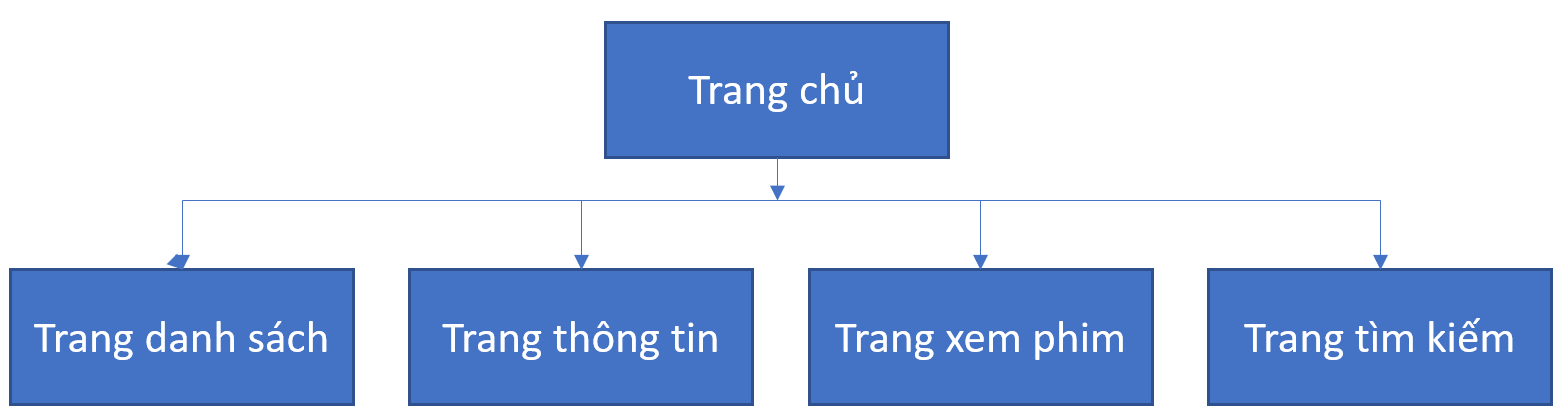
\includegraphics[scale=0.4]{31.png}
    \end{center}
    \caption{Sơ đồ của một trang web dành cho user}
    \label{refhinh1}
    \end{figure}
\end{center}

Đối với admin thì:

\begin{center}
    \begin{figure}[htp]
    \begin{center}
     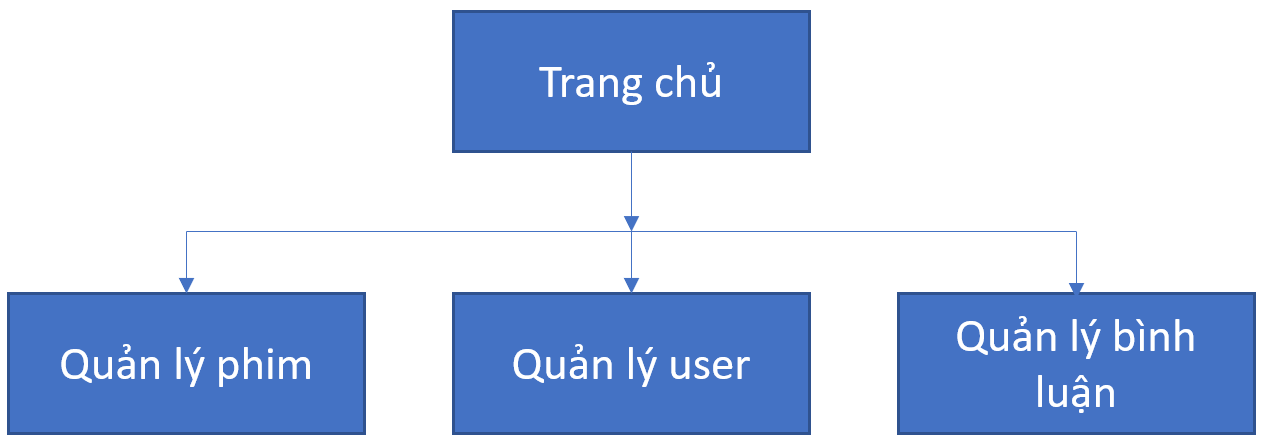
\includegraphics[scale=0.4]{32.png}
    \end{center}
    \caption{Sơ đồ của một trang web dành cho admin}
    \label{refhinh1}
    \end{figure}
\end{center}


\setlength{\parindent}{0cm}
\changefontsizes{14pt}
II. Xây dựng cơ sở dữ liệu

\setlength{\parindent}{1cm}
\changefontsizes{13pt}
Và cũng về cơ bản, cơ sở dữ liệu của một trang web xem phim gồm có các nội dung chính sau:

\begin{center}
    \begin{figure}[htp]
    \begin{center}
     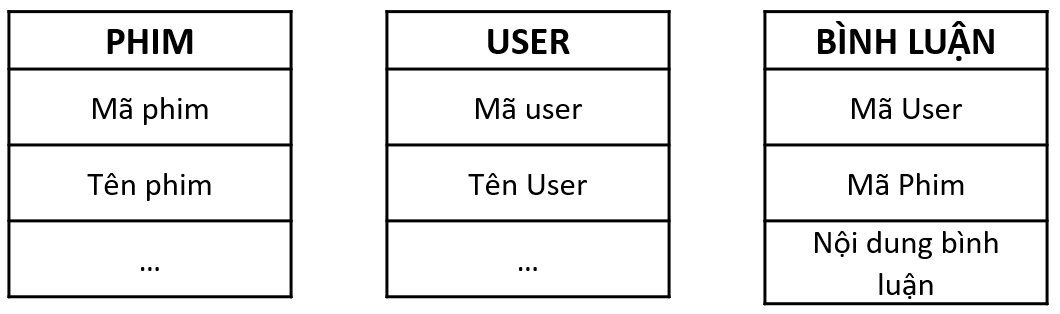
\includegraphics[scale=0.45]{33.png}
    \end{center}
    \caption{Cấu trúc của cơ sở dữ liệu}
    \label{refhinh1}
    \end{figure}
\end{center}


%Page ??
\newpage
\changefontsizes{16pt}
\centerline{\textbf{CHƯƠNG 4: HIỆN THỰC TRỰC QUAN HÓA}}


\setlength{\parindent}{0cm}
\changefontsizes{14pt}
I. Giao diện User

1. Cho phép user chọn phim theo từng thể loại, tìm kiếm phim

\changefontsizes{13pt}
\setlength{\parindent}{1cm}
User có thể tìm kiếm phim theo thể loại tại trang result.php

\begin{center}
    \begin{figure}[htp]
    \begin{center}
     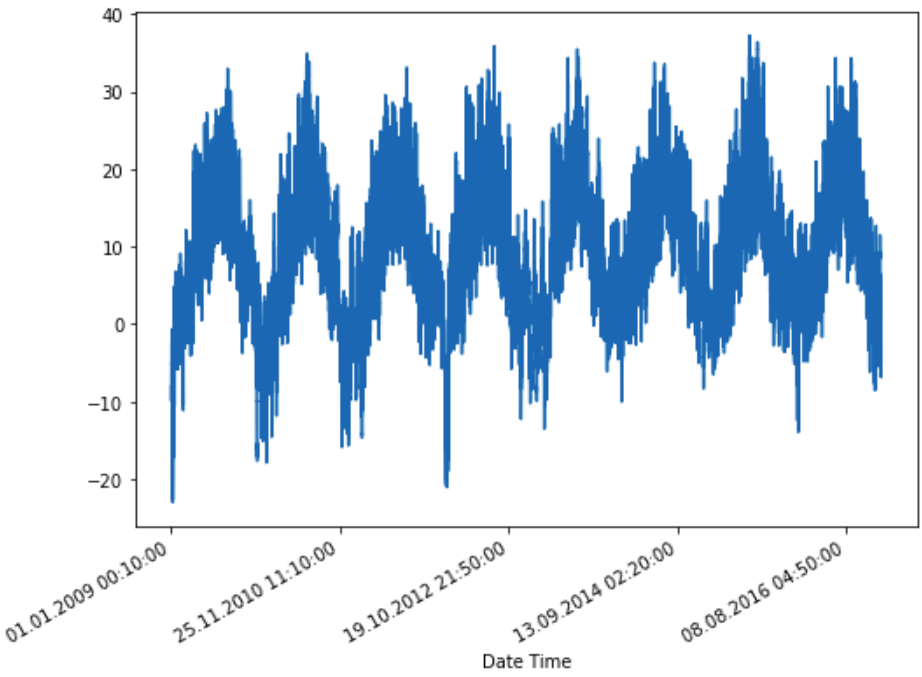
\includegraphics[scale=0.45]{1.png}
    \end{center}
    \caption{Giao diện trang result.php}
    \label{refhinh1}
    \end{figure}
\end{center}


User có thể tìm kiếm phim tại ô tìm kiếm và ấn nút tìm kiếm để bắt đầu tìm kiếm phim

\begin{center}
    \begin{figure}[htp]
    \begin{center}
     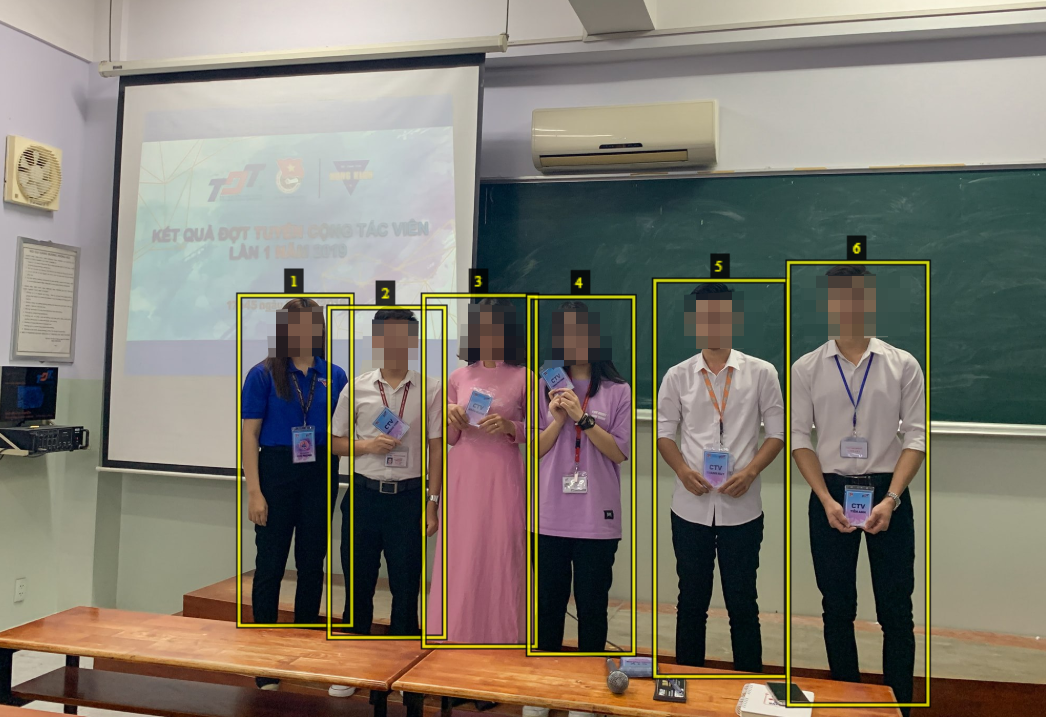
\includegraphics[scale=0.45]{2.png}
    \end{center}
    \caption{Giao diện trang search.php}
    \label{refhinh1}
    \end{figure}
\end{center}


\changefontsizes{14pt}
\setlength{\parindent}{0cm}
2. Trang chủ hiện các phim được đề cử, phim mới

\changefontsizes{13pt}
\setlength{\parindent}{1cm}
Tại trang chủ user có thể xem danh sách các phim mới và có thể xem phim đề cử bằng cách vào dòng chữ "Xem gì hôm nay."

\begin{center}
    \begin{figure}[htp]
    \begin{center}
     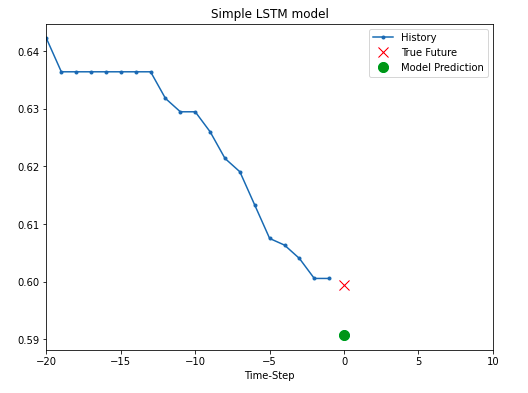
\includegraphics[scale=0.45]{3.png}
    \end{center}
    \caption{Giao diện trang hp.php}
    \label{refhinh1}
    \end{figure}
\end{center}

\changefontsizes{14pt}
\setlength{\parindent}{0cm}
3. Trang chi tiết hiện thông tin phim, diễn viên, đạo diễn, trailer, bình luận, đánh giá sao (rate), hiện các phim tương tự

\changefontsizes{13pt}
\setlength{\parindent}{1cm}
User có thể xem được các thông tin kể trên tại trang infor.php

\begin{center}
    \begin{figure}[htp]
    \begin{center}
     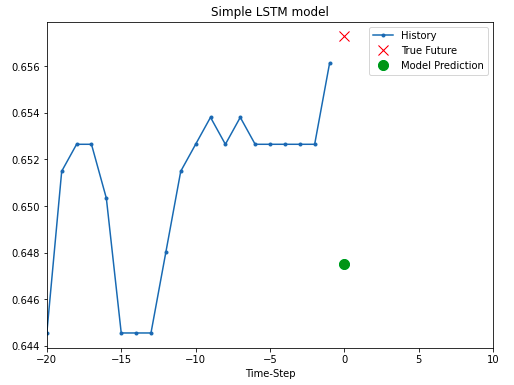
\includegraphics[scale=0.45]{4.png}
    \end{center}
    \caption{Giao diện trang infor.php}
    \label{refhinh1}
    \end{figure}
\end{center}

\newpage
\changefontsizes{14pt}
\setlength{\parindent}{0cm}
4. Nếu user đăng nhập thì cho phép bình luận và rating, bookmark các phim yêu thích

\changefontsizes{13pt}
\setlength{\parindent}{1cm}
Khi user đã đăng nhập, ví dụ với tài khoản User01 và mật khẩu 1234, user có thể đánh giá phim bằng cách chọn mức đánh giá ở phần "Đánh giá".

\begin{center}
    \begin{figure}[htp]
    \begin{center}
     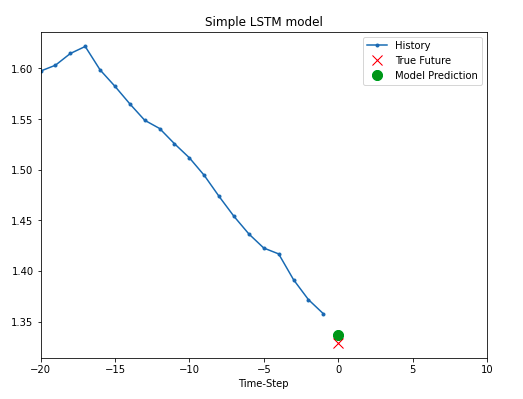
\includegraphics[scale=0.8925]{5.png}
    \end{center}
    \caption{Phần đánh giá phim tại trang infor.php}
    \label{refhinh1}
    \end{figure}
\end{center}

\newpage
Bình luận phim tại ô textbox

\begin{center}
    \begin{figure}[htp]
    \begin{center}
     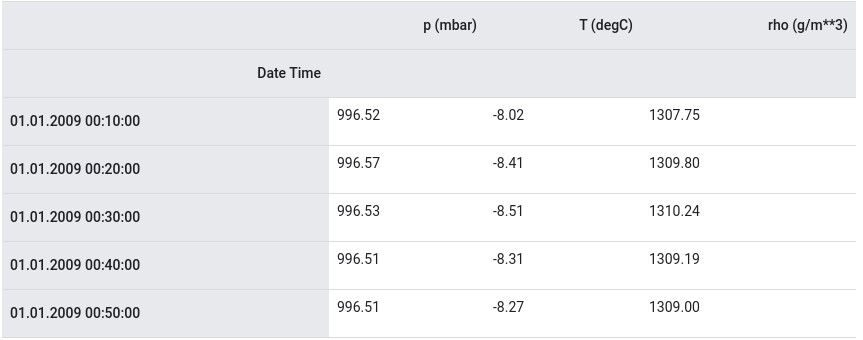
\includegraphics[scale=0.45]{6.png}
    \end{center}
    \caption{Phần bình luận phim tại trang infor.php}
    \label{refhinh1}
    \end{figure}
\end{center}

Lưu phim tại ô lưu

\begin{center}
    \begin{figure}[htp]
    \begin{center}
     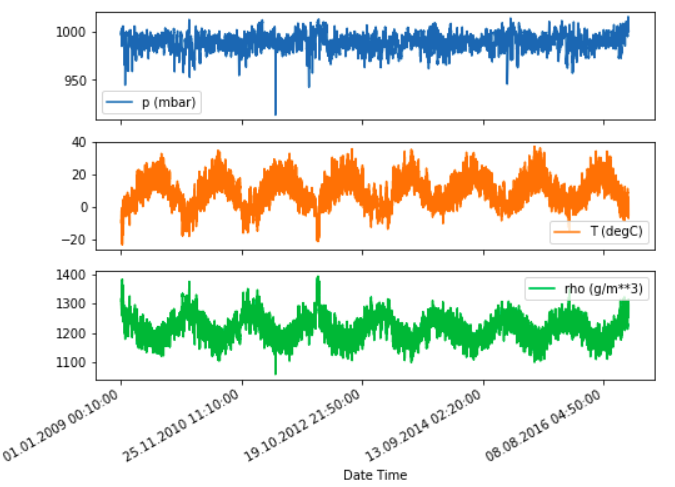
\includegraphics[scale=0.8]{7.png}
    \end{center}
    \caption{Phần lưu phim tại trang infor.php}
    \label{refhinh1}
    \end{figure}
\end{center}

%Page ??
\changefontsizes{14pt}
\setlength{\parindent}{0cm}
II. Giao diện Admin

1. Quản lý thể loại phim

\newpage
\bigskip
\changefontsizes{14pt}
\setlength{\parindent}{0cm}
2. Quản lý thông tin phim

\changefontsizes{13pt}
\setlength{\parindent}{1cm}
Admin quản lý thông tin phim tại trang Admin\_Listing.php

\begin{center}
    \begin{figure}[htp]
    \begin{center}
     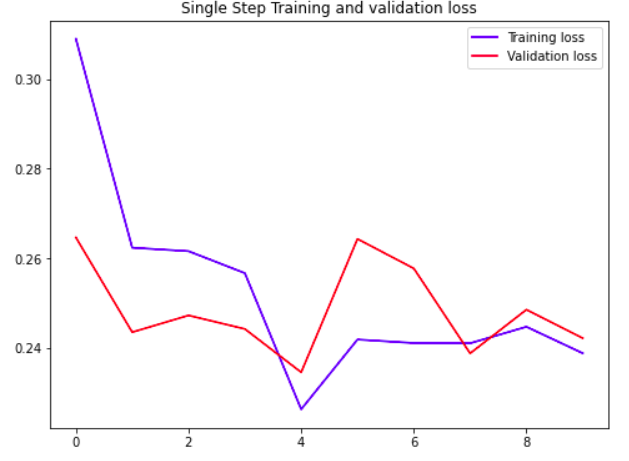
\includegraphics[scale=0.45]{8.png}
    \end{center}
    \caption{Giao diện trang Admin\_Listing.php}
    \label{refhinh1}
    \end{figure}
\end{center}

\bigskip
\changefontsizes{14pt}
\setlength{\parindent}{0cm}
3. Quản lý user

\changefontsizes{13pt}
\setlength{\parindent}{1cm}
Admin quản lý người dùng tại trang Manager\_User.php

\begin{center}
    \begin{figure}[htp]
    \begin{center}
     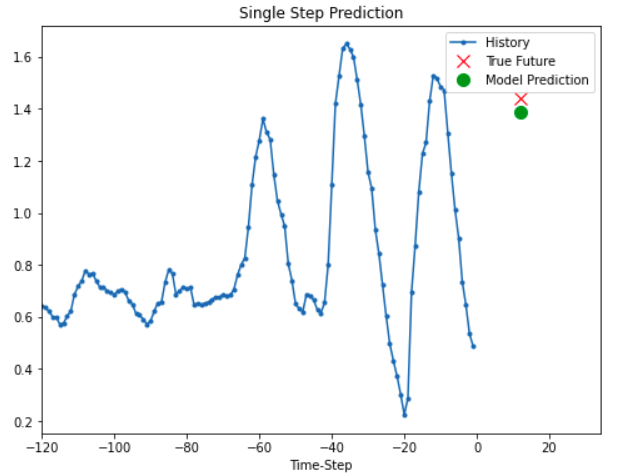
\includegraphics[scale=0.6]{9.png}
    \end{center}
    \caption{Giao diện trang Manager\_User.php}
    \label{refhinh1}
    \end{figure}
\end{center}

\bigskip
\changefontsizes{14pt}
\setlength{\parindent}{0cm}
4. Quản lý bình luận

\changefontsizes{13pt}
\setlength{\parindent}{1cm}
Admin quản lý bình luận của từng phim tại trang Manager\_Cmt.php

\begin{center}
    \begin{figure}[htp]
    \begin{center}
     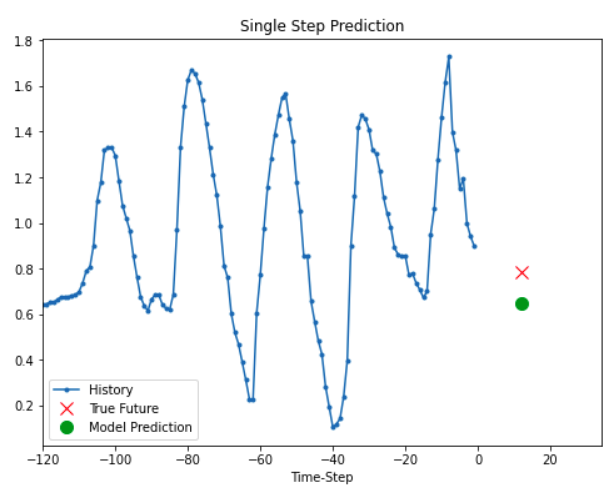
\includegraphics[scale=0.6]{10.png}
    \end{center}
    \caption{Giao diện trang Manager\_Cmt.php}
    \label{refhinh1}
    \end{figure}
\end{center}


.


%Page ??
\newpage
\changefontsizes{16pt}
\centerline{\textbf{CHƯƠNG 5: TỔNG KẾT}}

\bigskip
\changefontsizes{13pt}
\setlength{\parindent}{1cm}
Như vậy là chúng ta đã hoàn thành việc tạo dựng một trang web xem phim online. Đây chỉ là một trang web cơ bản nhưng nó đã thể hiện bao quát và gần như trọn vẹn nội dung mà sinh viên được học tại trường.

\newpage



\newpage
%Page ?? + 1
\newpage
\changefontsizes{16pt}
\centerline{\textbf{TÀI LIỆU THAM KHẢO}}

\vspace{1.2cm}
\changefontsizes{14pt}
\textbf{Tiếng Việt}

\bigskip
\setlength{\parindent}{1cm}

https://vi.wikipedia.org/wiki/HTML

https://vi.wikipedia.org/wiki/CSS

https://vi.wikipedia.org/wiki/JavaScript

https://vi.wikipedia.org/wiki/JQuery

https://vi.wikipedia.org/wiki/PHP

https://vi.wikipedia.org/wiki/XAMPP



\vspace{3cm}
\textbf{Tiếng Anh}




\end{document}